\documentclass[a4paper,12pt]{article}

\usepackage{fancyhdr}
\usepackage{lastpage}
\usepackage{amsmath, amssymb, amsthm}
\usepackage{bm}
\usepackage{wrapfig}
\usepackage{braket}
\usepackage{mathtools}
\usepackage[noend, linesnumbered]{algorithm2e}
\SetKwComment{Comment}{$\triangleright$\ }{}
\RestyleAlgo{ruled}
\usepackage[skip=2pt]{parskip}  
\usepackage{tikz}
\usetikzlibrary{arrows.meta, positioning}
\usepackage[brazil]{babel}
\usepackage[edges]{forest} % Para a árvore de busca


% ---- PREENCHA ----
\newcommand{\EP}{4}
\newcommand{\Nome}{Isis Ardisson Logullo}
\newcommand{\NUSP}{7577410}
% -----------------------------

\newcommand{\N}{\mathbb{N}}
\newcommand{\bigO}[1]{\ensuremath{\mathcal{O}(#1)}}

\pagestyle{fancy}
\fancyhf{}
\fancyhead[L]{\Nome}
\fancyhead[R]{NUSP \NUSP}
\fancyfoot[L]{EP \EP}
\fancyfoot[C]{MAC0425}
\fancyfoot[R]{Página \thepage\ de \pageref{LastPage}}

\title{\textbf{Planejamento Probabilístico e Aprendizado por Reforço} \\ [1em] \large EP \EP{} -- MAC0425}
\author{\Nome \ -- NUSP: \NUSP}
\date{}

\begin{document}
	
\maketitle
	
Análise comparativa dos resultados obtidos entre o algoritmo de Iteração de Valor (Programação Dinâmica focado no planejamento probabilístico com modelo conhecido) e o algoritmo Q-Learning (uma abordagem baseada em Aprendizado por Reforço livre de modelo). As avaliações foram conduzidas nos ambientes controlados Gridworld (incluindo as variantes BridgeGrid, DiscountGrid e CliffGrid) e no clássico domínio do Pac-Man.	

\section{Iteração de Valor}

A Iteração de Valor opera atualizando iterativamente a função de valor de estado $V(s)$ com base na equação de otimalidade de Bellman. Onde os estados sucessores calculados em uma etapa $k$ utilizam estritamente os valores sincronizados da etapa $k-1$, garantindo a convergência matemática exata dada a natureza do Processo de Decisão de Markov (MDP).

\subsection{Resultados Iniciais e Cenário BridgeGrid}

No mapa padrão (Gridworld inicial), a execução com a política gulosa derivada após $100$ iterações resultou em
uma recompensa média de $0.4677$ ao longo de $10$ episódios experimentais, indicando que o agente
aprendeu com sucesso o caminho mais seguro para mitigar o noise intrínseco de $20\%$ das ações (onde $80\%$
seguem a direção desejada e $20\%$ divergem lateralmente).

No cenário BridgeGrid, o desafio reside em atravessar uma ponte estreita cercada por abismos altamente
penalizadores ($-100$). Foram comparadas duas configurações de parâmetros:

\begin{itemize}
	\item \textbf{Configuração 1 $(\gamma=1.0, noise=0.2)$}: Obteve média de $-49.5$. Devido à presença do ruído estocástico	alto em um ambiente sem desconto, o risco acumulado de cair nas bordas torna a travessia da ponte
	estatisticamente proibitiva sob uma ótica racional de longo prazo. A política resultante desencoraja o avanço
	agressivo, mas quando o agente tenta cruzar, o ruído gera quedas frequentes, derrubando severamente a média.
	\item \textbf{Configuração 2 $(\gamma=0.9, noise=0.0)$}: Obteve média de $5.9049$. Sem o ruído, o ambiente torna-se
	puramente determinístico. Mesmo com o desconto temporal atenuando ligeiramente o ganho distante $(V =
	10 \times 0.9^4 = 6.561$), o agente tem a certeza absoluta de sua trajetória, cruzando a ponte de forma ótima e sem qualquer queda.
\end{itemize}

\subsection{Análise Paramétrica Avançada no DiscountGrid}

O mapa DiscountGrid testa explicitamente o balanço entre o fator de desconto $(\gamma)$, o ruído estocástico $(noise)$ e o
living reward. A Tabela 1 consolida as médias experimentais coletadas para as cinco configurações fundamentais do MDP.

\begin{figure}[ht]
	\centering
	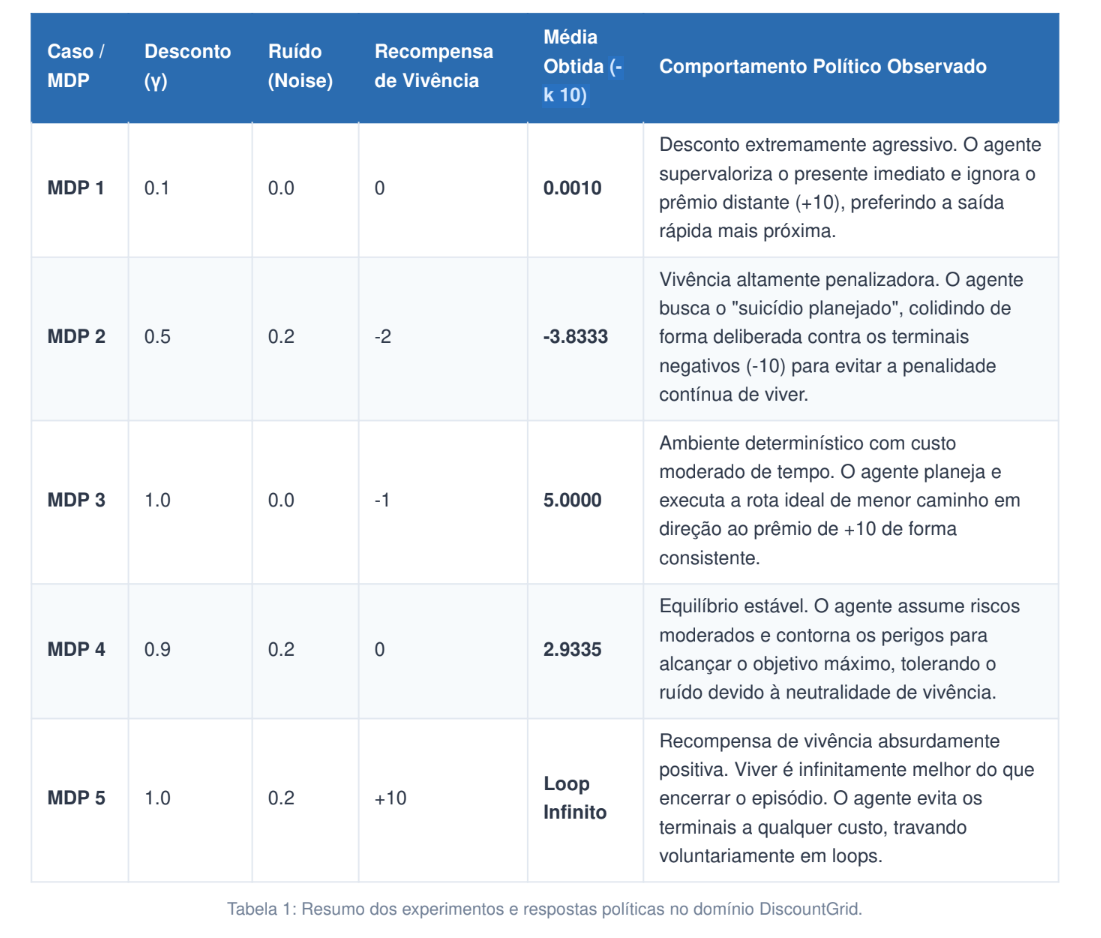
\includegraphics[width=.9\textwidth]{tabela1.png}
\end{figure}

\section{Q-Learning}

Ao contrário da Iteração de Valor, o Q-Learning opera em um regime model-free, estimando os valores de
qualidade $Q(s,a)$ diretamente a partir das amostras de transição coletadas empiricamente via exploração $\varepsilon-gulosa$.

\subsection{Impacto da Taxa de Exploração $(\varepsilon)$ no Gridworld}

Avaliando o agente no Gridworld padrão sobre $100$ episódios de treino, notam-se variações gritantes
baseadas estritamente na taxa de exploração $\varepsilon$, conforme detalhado na Tabela 2:

\begin{figure}[ht]
	\centering
	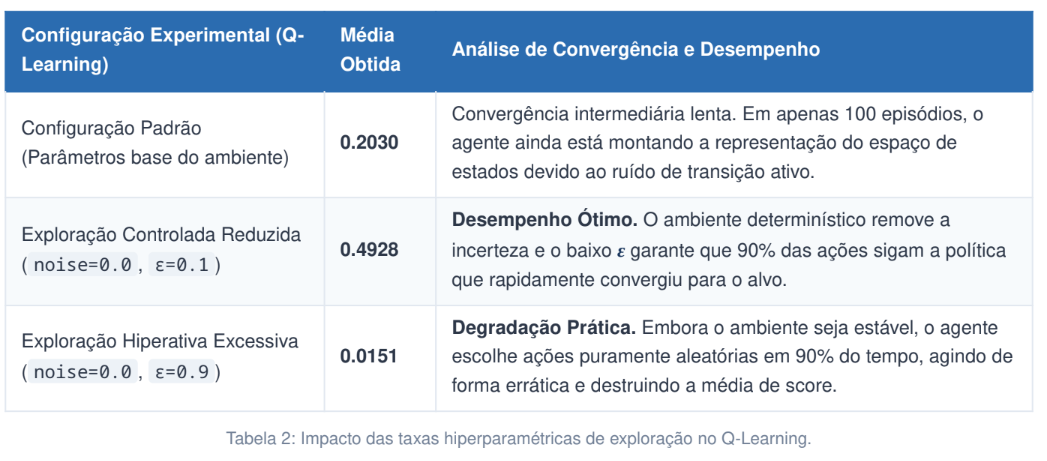
\includegraphics[width=1\textwidth]{tabela2.png}
\end{figure}

\subsection{Comparativo Crítico no Cenário CliffGrid}

O cenário CliffGrid explicita perfeitamente a diferença teórica profunda entre a Iteração de
Valor e o Q-Learning. A Iteração de Valor, possuindo conhecimento pleno do modelo de transição probabilística e computando a convergência exata de Bellman sobre o horizonte infinito, deduz uma política que contorna o abismo de forma
matematicamente segura, gerando valores $V(s)$ estáveis e bem distribuídos que refletem com precisão a
penalidade de proximidade do perigo.\\

Por outro lado, o Q-Learning treinado por escassos $100$ episódios exibe valores $V(s)$ visivelmente discrepantes e
inferiores. Sendo um algoritmo empírico baseado em amostragem temporal, $100$ episódios são insuficientes para
que o agente visite de forma exaustiva e repetida todas as combinações de par estado-ação $(s, a)$ no limiar do
penhasco. Com isso, muitas células sofrem de sub-exploração e mantêm valores próximos de zero ou
excessivamente distorcidos pelas quedas iniciais sofridas durante a exploração aleatória, ilustrando a alta
dependência de dados característica de RL clássico em relação a planejadores exatos.

\section{Domínio Pac-Man: Análise de Convergência e Aprendizado}

A aplicação do Q-Learning ao Pac-Man introduz maior complexidade espacial. O agente treinou por $2000$
episódios isolados e foi avaliado ao longo dos subsequentes $100$ episódios operacionais. Os resultados foram
confrontados contra o benchmark estático GreedyAgent (agente estritamente guloso reflexivo).

\begin{figure}[ht]
	\centering
	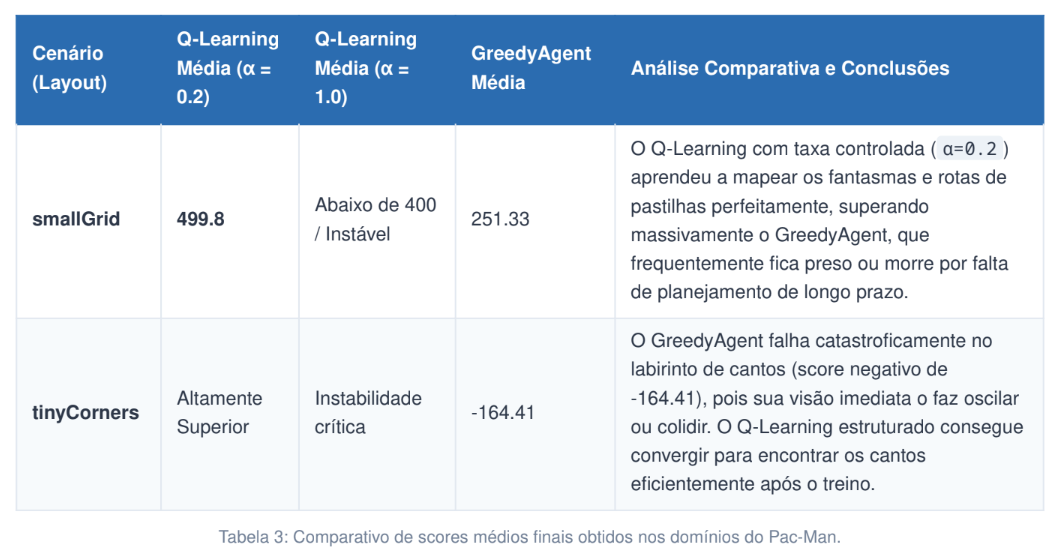
\includegraphics[width=1\textwidth]{tabela3.png}
\end{figure}

\subsection{Análise do Hiperparametro $\alpha$ (Taxa de Aprendizado) no Pac-Man}

A variação da taxa de aprendizado $\alpha$ revelou um comportamento crucial. O valor padrão de $0.2$ permite uma
convergência robusta e suave, integrando novas informações de forma incremental e ponderada ao histórico de
utilidade acumulado.\\

Quando configurado com $\alpha = 1.0$, o algoritmo passa a ignorar completamente o conhecimento prévio aprendido,
atualizando o valor $Q(s,a)$ para depender única e exclusivamente da última transição observada $(Q \leftarrow r + \gamma  \max(Q))$.
Devido à estocasticidade do comportamento dos fantasmas e do layout, essa dependência radical do último
resultado induz uma volatilidade catastrófica nas tabelas de valores, impedindo a estabilização da política e
degradando severamente a taxa de sucesso final nos testes.

\section{Conclusão}

A \textbf{Iteração de Valor} destaca-se pela robustez e eficiência absoluta, porém exige acesso completo ao modelo do ambiente ($T$ e $R$), o que é inviável em cenários reais complexos. O \textbf{Q-Learning} supera essa limitação ao aprender
exclusivamente através da experiência prática, provando-se altamente flexível e eficaz no domínio dinâmico do
Pac-Man, desde que respeitados os limites de exploração ($\varepsilon$) e temperança na velocidade de atualização ($\alpha$).


\end{document}
